\documentclass{article}
\usepackage{../fasy-hw}

%% UPDATE these variables:
\renewcommand{\hwnum}{3}
\title{Computational Topology, Homework \hwnum}
\author{\todo{your name(s) here}}
\collab{\todo{list your collaborators here}}
\date{due: 3 March 2022 (accepted through 7 March 2022)}

\begin{document}

\maketitle

\input{../directions}

\nextprob{Arrangements}
% \collab{TODO - uncomment if your collaborators on this have changed

This homework can be handed in as a group or as individual.
Suppose that we have a set $\mathcal{L}$ of non-vertical lines in general position (by
\emph{general position} here, we mean that no two lines are
parallel and no three share a common point).
Since no line is vertical, we can think of each line as an oriented line, going
from left to right.  Then, `above' the line follows the right-hand rule and is
consistent with our intuition for `above.'  Suppose we also have
a path $p$  that originates below all lines and crosses each
line exactly once as it goes `up'.  Add a line at infinity that intersects
all other lines to the right of all intersections.  The following steps will
visit all intersections in this arrangement that are to the right of the path.

\begin{enumerate}[(a)]
    \item Define an \emph{upper horizon tree} by starting with the edges of the
        arrangement that cross the path (note that each edges inherits a
        direction from the line, so will be oriented from left to right). At each vertex where
        two edges collide, only the upper edge continues, as shown in pink in
        \figref{arrangement}. Give an algorithm to
        compute the upper horizon tree in $\Theta(n \log n)$ time.
    \item Prove that if there are any arrangement vertices to the right of the
        path, then there is a triangle formed by the path and two edges of the
        upper horizon tree.  Prove also that the uppermost triangle (labeled
        $A$ in the \figref{arrangement}) is also a triangle of the arrangement
        $\mathcal{L} \cup p$.  (Note that
        the triangle labeled $B$ is not).
    \item We can advance the path past the uppermost triangle so that the two edges swap
        order along the path.  Describe how to update the horizon tree to become
        the upper horizon tree for this modified path.
    \item If we keep triangles in a stack, we can always have
        access to the uppermost triangle.  How do we maintain this stack when we
        advance past a triangle?
    \item Show that the total time spent maintaining the upper horizon tree is
        $O(n^2)$.  Hint: you can apply the Zone Theorem (Theorem 8.5 of the
        Dutch book) to each line in the arrangement.
\end{enumerate}

Note: this HW assignment was borrowed from the Computational Geometry class that
I took at University of North Carolina with Jack Snoeyink.  Thanks, Jack!

\begin{figure}[bht]
    \centering
    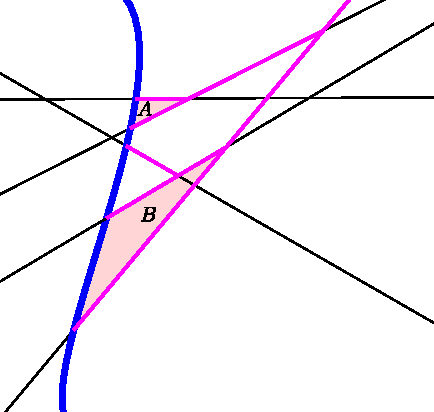
\includegraphics[height=3in]{arrangement}
    \caption{Arrangement of five lines in the plane (black lines), and a path
    (bold blue).}\label{fig:arrangement}
\end{figure}

\end{document}
